% Insert after the new validation-fraction subsection.
\subsection{Sensitivity to Array Position Errors}
\label{sec:revision-position-mismatch}

To test one departure from the ideal ULA model, we perturb the element
positions according to
\begin{equation}
\frac{x_n}{\lambda}=\frac{n-1}{2}+s_x u_n,
\qquad u_n\sim\mathcal N(0,1),
\end{equation}
with independent $u_n$ and $s_x\in\{0,0.005,0.01,0.02\}$.
These are declared stress levels,
not measured hardware tolerances. The estimator continues to apply its
ULA Hankel processing, and channel error is measured against the actual
perturbed channel. The reference field remains known and calibrated.

We use $N=32$, $K=3$, $P=30$, SNR $=5$~dB, RSR $=12$~dB and
$L\in\{3,12\}$ paths per user. Each setting uses 400 paired trials and
the same 100/25 update counts, four sweeps and 30\% validation fraction.
For a given trial, the path parameters, pilots, thermal-noise draw and
normalized offsets $u_n$ are shared across the four strengths. We do not
renormalize the realized channel after perturbing the positions; SNR
retains its nominal statistical-power definition.

As shown in Fig.~\ref{fig:revision-position}, the HS-GS gain decreases
as the position errors increase. For $L=3$, its ratio-of-sums gain over
EM-GS changes from $4.955$~dB without mismatch to $3.917$~dB at
$s_x=0.02$, with interval $[3.748,4.075]$~dB at the latter point.
For $L=12$, the gain decreases from $0.264$ to $0.050$~dB; the final
interval, $[-0.029,0.125]$~dB, includes zero. Thus, the tested sparse
case retains a benefit, while the smaller benefit in the more complex
case becomes uncertain. This experiment does not establish robustness to
unknown reference calibration, mutual coupling, near-field propagation
or correlated noise.

\begin{figure*}[!t]
\centering
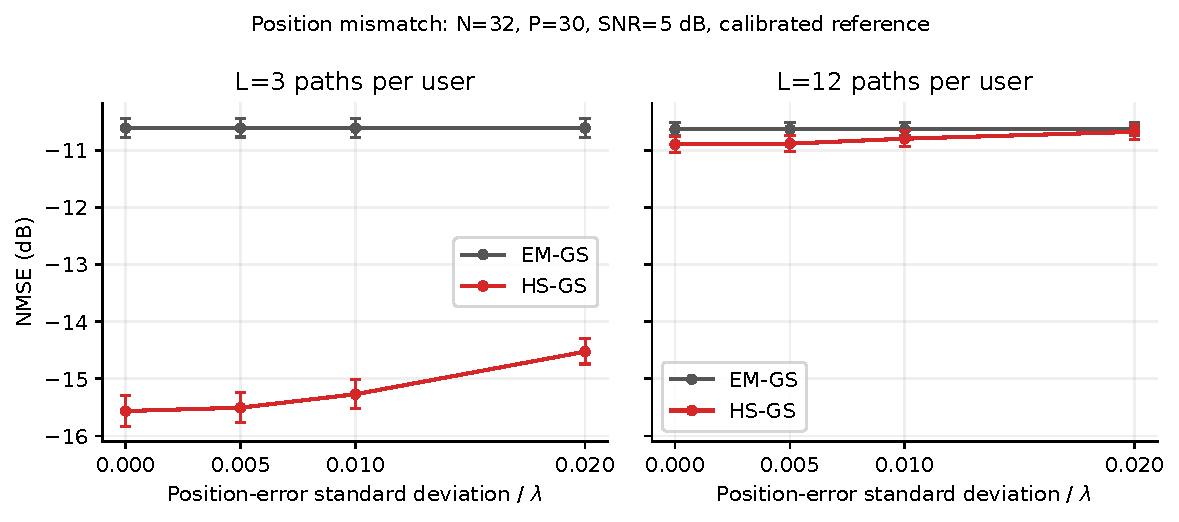
\includegraphics[width=\textwidth]{fig/revision_position_mismatch.pdf}
\caption{Position-error stress test with a known calibrated reference and
the actual perturbed channel as the estimation target. Each point uses
400 trials; trials are paired across mismatch strengths within each path
count. Error bars are pointwise 95\% paired-bootstrap intervals from
4,000 resamples.}
\label{fig:revision-position}
\end{figure*}
